\documentclass[00_complete]{subfiles}

%\documentclass[12pt]{report}
\usepackage[utf8]{inputenc}
\usepackage{amsmath,amssymb,amsthm,gensymb,parskip,graphicx,footmisc,csquotes,enumerate,datetime2}
\usepackage[]{libertinus}
\usepackage[breaklinks]{hyperref}
\hypersetup{
  pdfauthor={Moshe Krumbein},
  colorlinks=true,
  linkcolor={black},
  filecolor={black},
  citecolor={black}, %blue
  urlcolor={black}, %blue
}
\usepackage[top=30mm,bottom=30mm,left=30mm,right=30mm]{geometry}
%\setlength{\emergencystretch}{2em} % prevent overfull lines
\providecommand{\tightlist}{%
\setlength{\itemsep}{0pt}\setlength{\parskip}{0pt}}

\renewcommand\qedsymbol{$\blacksquare$}

\theoremstyle{definition}
\newtheorem*{definition}{Definition}
\newtheorem*{theorem}{Theorem}
\newtheorem*{axiom}{Axiom}
\newtheorem*{lemma}{Lemma}

\theoremstyle{remark}
\newtheorem*{note}{Note}
\newtheorem*{symbols}{Symbol}
\newtheorem{example}{Example}[section]
\newtheorem*{claim}{Claim}
\newtheorem*{conclusion}{Conclusion}
\newtheorem*{reminder}{Reminder}

\usepackage{fancyhdr}
\usepackage[italicdiff]{physics}
\MakeOuterQuote{"}

\renewcommand{\chaptermark}[1]{\markboth{#1}{}}

\pagestyle{fancy}

\setlength{\headheight}{14.5pt}
\addtolength{\topmargin}{-2.5pt}

\fancyhf{}
\rhead{Moshe Krumbein}
\lhead{\chaptermark}
\cfoot{\thepage}
\fancyhead[R]{\chaptername~\thechapter}
\fancyhead[L]{\mbox{\leftmark}}

\usepackage[Rejne]{fncychap}
\usepackage{titling}

\makeatletter
\renewcommand{\@chapapp}{\vspace*{-100pt}\huge\thetitle}
\makeatother

\makeatletter
\newcommand{\subtitle}[1]{%
  {\center\vspace*{-60pt}%
  \linespread{1.1}\Large\scshape#1%
  \par\nobreak\vspace*{35pt}}
}
\makeatother

\newcommand{\Chapter}[2]{
    \def\n{#2}
    \setcounter{chapter}{\the\numexpr\n-1}
    \chapter{#1}
    \subtitle{\theauthor~- \thedate}
}

\DeclareMathOperator{\Ima}{Im}
\DeclareMathOperator{\Id}{Id}
\DeclareMathOperator{\cis}{cis}

\newcommand{\Mod}[1]{\ (\mathrm{mod}\ #1)}
\newcommand{\st}[0]{\;\mathrm{s.t.}\;}

\title{Discrete Mathematics}
\author{Moshe Krumbein}
\date{Fall 2021}

\begin{document}
\Chapter{Graph Theory}{11}

\section{Introduction}
\begin{definition}[(Undirected) Graph]
    Is a order pair $G=(V,E)$ such that:
    \begin{enumerate}
        \item[$V$ -] Set of vertices - finite and not empty.
        \item[$E$ -] Set of edges - collection of the unordered pairs of
            distinct elements of $V$.
    \end{enumerate}
    Given $u,v \in V$, if $\{u,v\} \in E$ we can also write $(u,v) \in E$ (even
    though in general we reserve parentheses for ordered pairs).
\end{definition}
\begin{example}
    \label{one}
    \begin{figure}[ht]
        \centering
        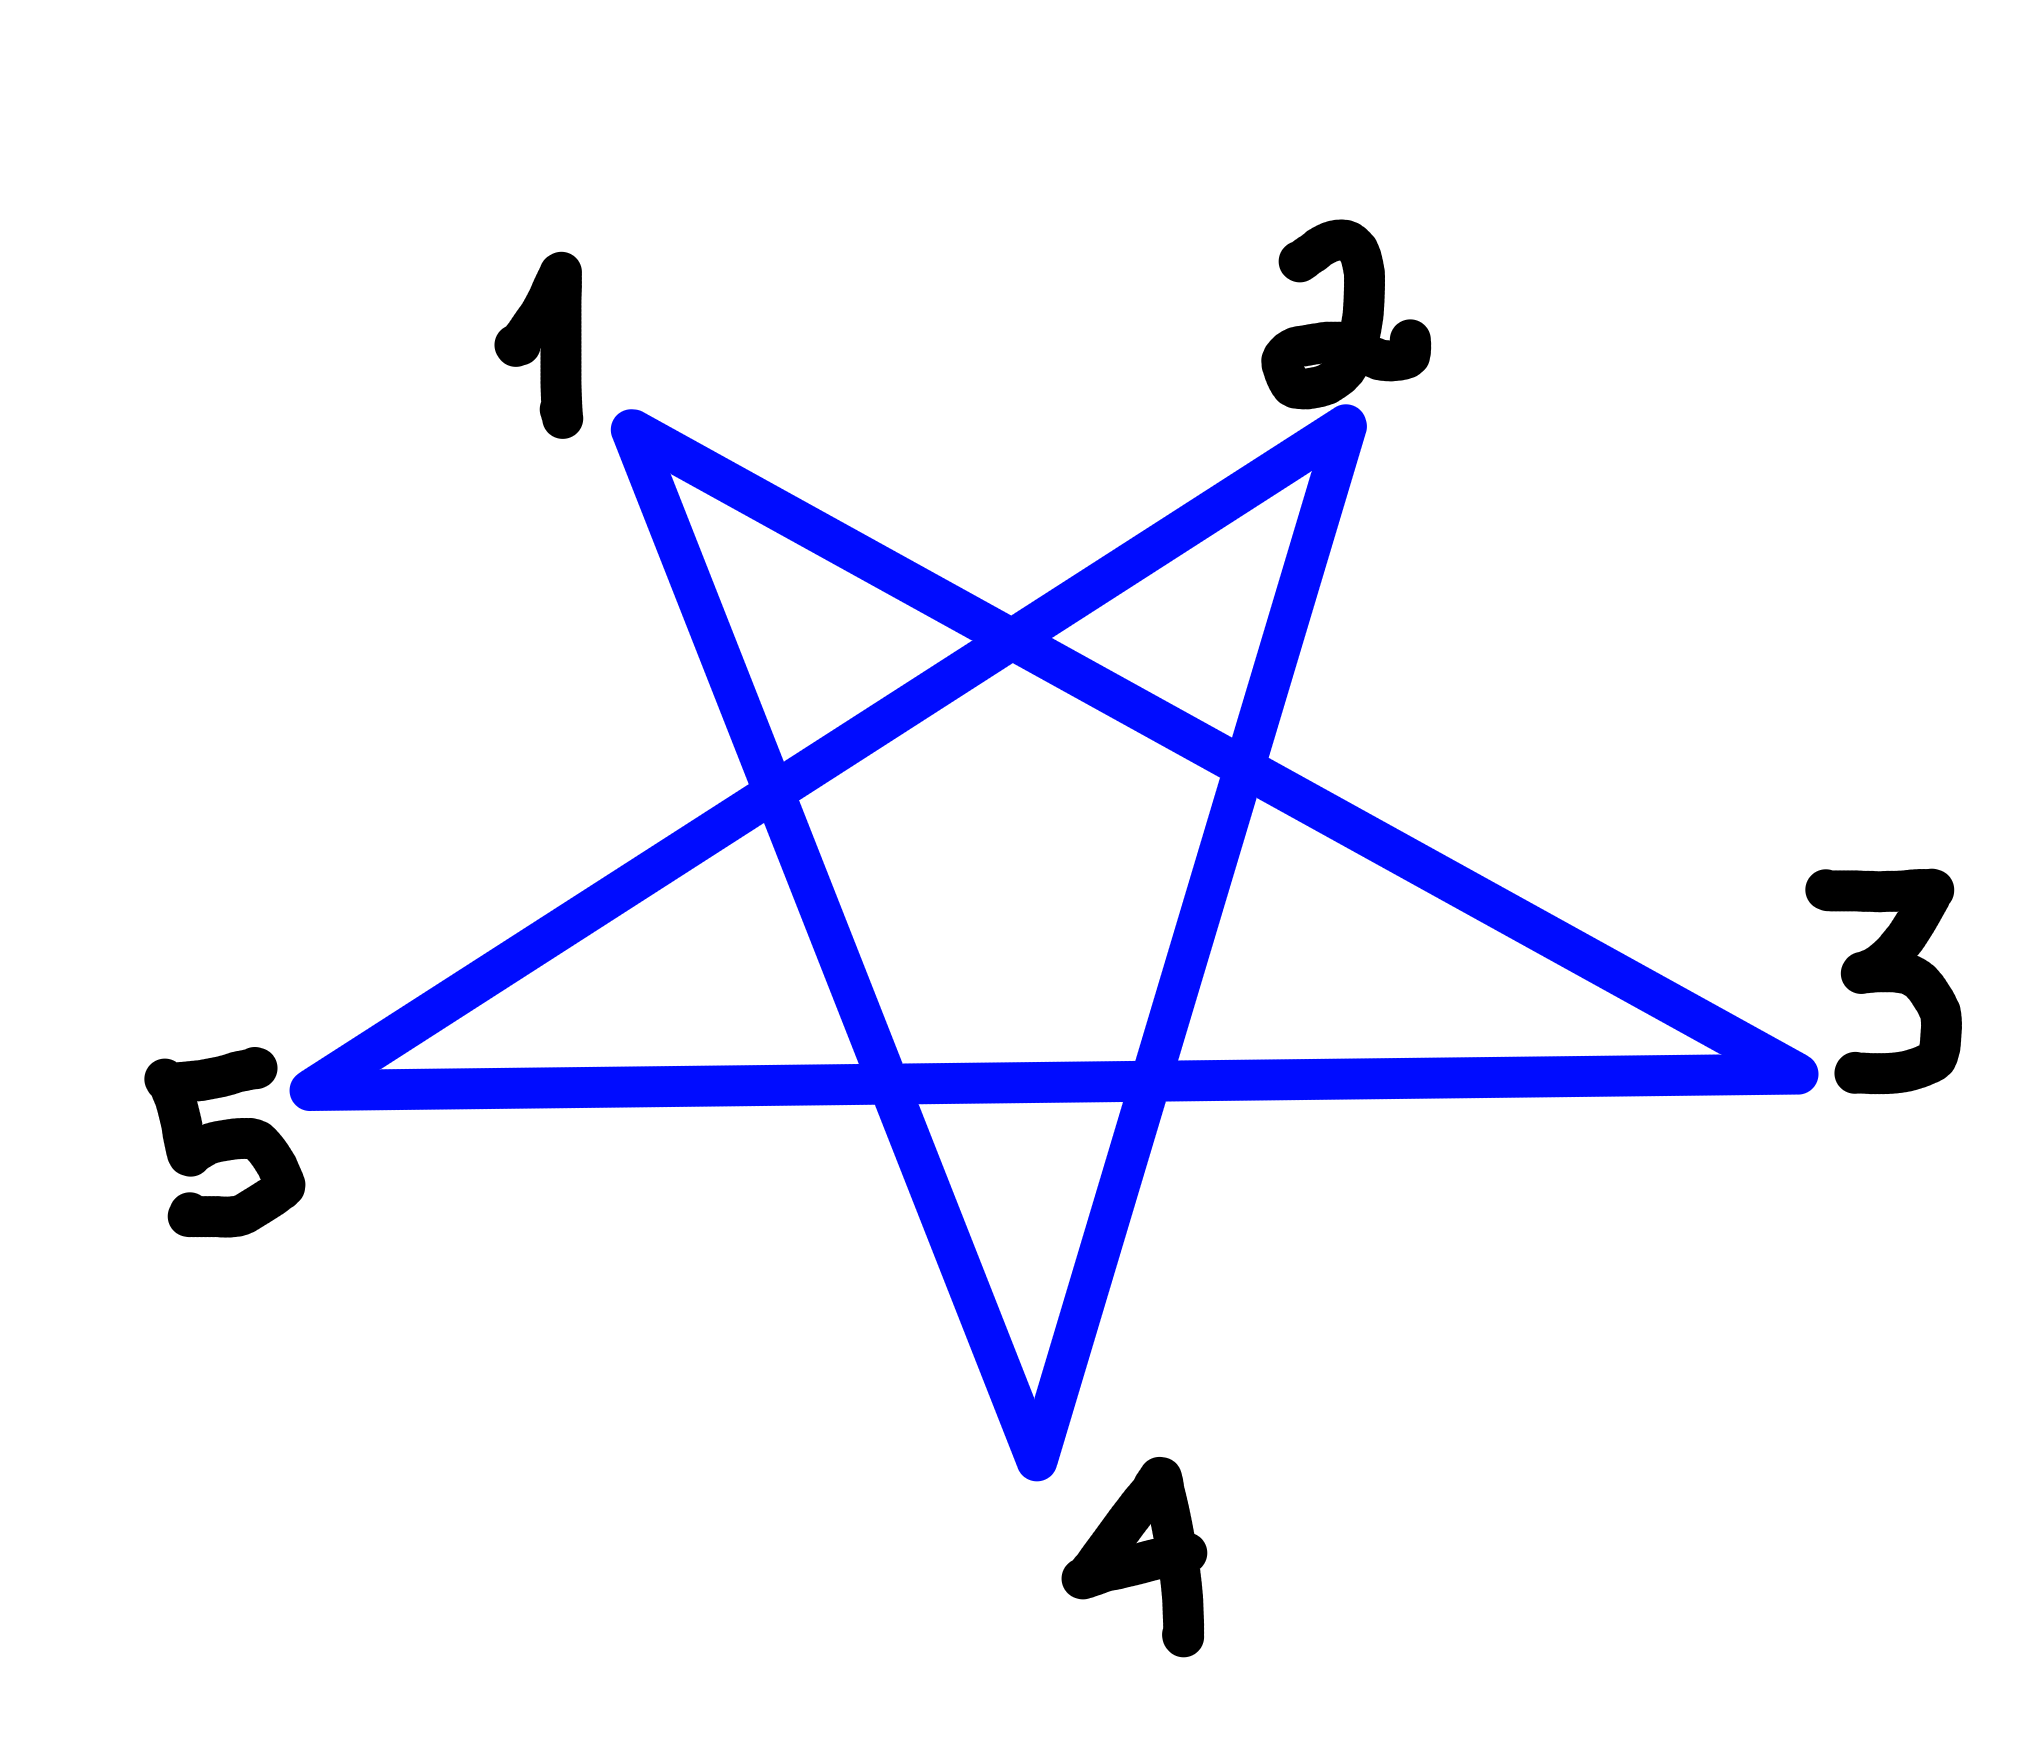
\includegraphics[width=0.33\textwidth]{w11_1}
        \caption{Example \ref{one}}
    \end{figure}
    \begin{gather*}
        V= \{1,2,3,4,5\} \\
        E=\{(1,3),(3,5),(5,2),(2,4),(4,1)\}
    \end{gather*}
    \begin{table}[ht!]
    \centering
    {\renewcommand{\arraystretch}{1.2}% for the vertical padding
    \begin{tabular}{c|ccccc}
    & 1 & 2 & 3 & 4 & 5 \\
    \hline
        1 &0&0&1&1&0 \\
        2 &0&0&0&1&1 \\
        3 &1&0&0&0&1 \\
        4 &1&1&0&0&0 \\
        5 &0&1&1&0&0 \\
\end{tabular}}
\caption{Example \ref{one}}
\end{table}
\end{example}
\section{Special Graphs}
\begin{definition}[Empty/Null Graph ($N_n$)]
    $$|V|=n \quad E=\emptyset$$
\end{definition}
\begin{definition}[Complete Graph ($K_n$)]
    $$|V|=n \quad E=\{(i,j) \mid 1 \leq i < j \leq n\}$$
    $$|E|=\binom{n}{2}$$
\end{definition}
How may different graphs are there with $n$ vertices?

Every subset of the complete graph produces a different graph:
$$2^{\binom{n}{2}}$$
\begin{definition}[Circle Graph ($C_n$)]
    $$|V|=n \quad E=\{(1,2),(2,3),\dots,(n-1,n),(n,1)\}$$
    $$|E|=n$$
\end{definition}
\begin{definition}[Neighbors]
    Given $u,v \in V$ $u$ and $v$ are \emph{neighbors} if $(u,v) \in E$.
\end{definition}
\begin{definition}[Degree of a Vertex]
    The \emph{degree} of a vertex $u \in V$ is the number of \emph{neighbors}
    of $u$.
    $$\deg(u) = |\{v \in V \mid (u,v) \in E\}|$$
\end{definition}
\begin{claim}
    The sum of the degrees of all the vertices in a graph is equal to $2|E|$.
    In other words:
    $$\sum_{v \in V}\deg(v) = 2|E|$$
\end{claim}
\begin{proof}
    We will symbolize for all $v \in V$, $e \in E$:
    $$T(e,v) = \begin{cases}
        1 & v \in e \\
        0 & v \notin e
    \end{cases}$$
    \begin{gather*}
        \sum^{v \in V}\deg(v) = \sum_{v \in V}\sum_{e \in E} T(e,v)= \sum_{e
        \in E}\underbrace{\sum_{v \in V} T(e,v)}_{2}=\sum_{e \in E}2=2|E|
    \end{gather*}
\end{proof}
\begin{conclusion}
    The number of vertices that have have an odd degrees is even.
\end{conclusion}
\begin{definition}[Path]
    A \emph{path} in graph $G=(V,E)$ is a sequence of vertices $(v_0,v_1,
    \dots, v_n)$ such that for all $0 \leq i \leq n-1$: $(v_i,v_{i+1}) \in E$,
    which has a length of $n$.
\end{definition}
\begin{definition}[Connectivity]
    Graph $G=(V,E)$ is \emph{connected} if for all $u,v \in V$ there exists a
    \emph{path} $(v_0,v_1,\dots,v_n)$ such that $v_0=u$ and $v_n=v$.
\end{definition}
\begin{definition}[Components]
    We define relation $R$ on $V$:

    $(u,v) \in R \iff$ there exists a path $(v_0,\dots,v_n)$ in the graph such
    that $v_0=u$ and $v_n=v$.
    \begin{note}
    For all $v \in V$: $(v)$ is a path.
\end{note}
\begin{claim}
    This relation is an equivalence relation of $V$.
\end{claim}
\end{definition}
These equivalence classes are called \emph{connected components} of $G$.
\begin{claim}
    If $G$ is \emph{connected}, then the relation on $V$ is the full/complete
    relation (in other words, for all $u,v \in V, (u,v) \in R$), and therefore
    we get one \emph{connected component}.

    For the empty graph $N_n$, we get $n$ \emph{components}.
\end{claim}
\begin{claim}
    The number of components in a graph $G=(V,E)$ is greater or equal to
    $|V|-|E|$.
\end{claim}
\begin{proof}
    Induction of the number of edges.
    \begin{enumerate}[I.]
        \item $|E|=0$: Number of components $=n=|V|-|E|$
        \item We assume induction for $|E|=k$ and we'll prove for $|E|=k+1$:
        Our graph is $G=(E,v)$, $|V|=n$ and $|E|=k+1$. We'll pick $e \in E$ and
        we'll define $G_0=(V,E\setminus\{e\})$, which is a graph with $n$
        vertices and $k$ edges.

        From the initial assumption, the number of components in $G_0 \geq
        n-k$.

        Suppose $e=(u,v)$. If in $G_0$, $u$ and $v$ belong to the same
        component, then the number of components in $G =$ the number of
        components in $G_0 \geq n-k > n-k-1$.

        If $u$ and $v$ are not in the same component in $G_0$, then the number
        of components in $G =$ number of components in $G_0-1 \geq n-k-1 =
        n-(k+1)$.
    \end{enumerate}
\end{proof}
\begin{definition}[Simple Path]
     A path $(v_0,\dots,v_n)$ is called a \emph{simple path} if all the
     vertices $v_0,\dots,v_n$ are different from each other.
\end{definition}
\begin{definition}[Simple Circuit]
    A path $(v_0,\dots,v_n)$ is called a \emph{simple circuit} if
    $v_1,\dots,v_n$ are all different and $v_1=v_n$ (where $n\geq3$).
\end{definition}

\section{Trees}
\begin{definition}[Tree]
    A connected graph without any \emph{simple circuits} is called a
    \emph{tree}.

    $v$ is a \emph{leaf} (external vertex) if $\deg(v)=1$.
\end{definition}
\begin{lemma}
    Any \emph{tree} that has more than one \emph{vertex} has at least one
    \emph{leaf}.
\end{lemma}
\begin{proof}
    Given a tree $G=(V,E)$ and $v_0 \in V$. $\deg(v_0) \neq 0$, because that
    would with violate the requirement that trees are \emph{connected} or the
    condition of having more than one vertex of the initial claim.

    If $\deg(v_0)=1$, we found a \emph{leaf}.

    If $\deg(v_0)>1$ than it has part of a path that has an end vertex $v_n$
    such that $\deg(v_n)=1$ (because there are no circuits in trees).
\end{proof}
\begin{claim}
    If $G=(V,E)$ is a tree, then $|V|-|E|=1$.
\end{claim}
\begin{proof}
   Proof by induction on the number of vertices in the graph:
   \begin{enumerate}[I.]
       \item $|V|=0$, and therefore $E = \emptyset$, and therefore
           $|V|-|E|=1-0=1$.
       \item We assume $|V|=n$ works, and we proof $|V|=n+1$ also works:

        As per the aforementioned lemma, there exists a leaf $v \in V$.

        Let there be $e \in E$ such that $v\in e$. We then define
        $G'=(V\setminus\{v\},E\setminus \{e\})$. We see that $G'$ is a tree
        because it doesn't contain any \emph{simple circuits} and is
        \emph{connected}, because we removed only a \emph{leaf} and its edge.

        In addition, $G'$ has $n=|V|-1$ vertices and $|E|-1$ edges. Therefore, $G'$
        fulfills the assumption of induction and therefore:
        $$|V|-|E|=(|V|-1)-(|E|-1)=|V\setminus\{v\}|-|E\setminus\{e\}|=1$$
   \end{enumerate}
\end{proof}
\begin{claim}
    Given graph $G=(V,E)$ without \emph{simple circuits} such that
    $|V|-|E|=1$, then $G$ is \emph{connected}.
\end{claim}
\begin{proof}
    $V_1,V_2,\dots V_l$ are \emph{connected components} of G.

    For all $1 \leq i \leq l$:
    $$E_i=\{\{u,w\}\in E \mid u,w \in V_i\}$$
    Because \emph{components} are \emph{equivalence classes}, we know that
    $E_i\cap E_j=\emptyset$ and $E_1\cap E_2 \cap \dots \cap E_l=E$. From here
    we see that $|E_1|+|E_2|+\dots+|E_l|=|E|$.

    In addition, for all $1 \leq i \leq l$, the graph $G_i=(V_i,E_i)$ is a tree
    because it is \emph{connected} and doesn't have any \emph{simple circuits}.
    Therefore, as per the previous claim, $|V_i|-|E_i|=1$.
    \begin{gather*}
    1=|V|-|E|=(|V_1|+\dots+|V_l|)-(|E_1|+\dots+|E_l|)=(|V_1|-|E_1|)+\dots+(|V_l|-|E_l|)
    \\
    =\underbrace{1+1+\dots+1}_{l \text{ times}}=l \implies l=1
    \end{gather*}
    Therefore, $G$ has only one \emph{connected component}, meaning $G$ is
    \emph{connected}.
\end{proof}
\begin{claim}
    If $G=(V,E)$ is a \emph{connected} graph and $(v_0,\dots,v_n)$ is a
    simple circuit in $G$, then $G'=(V,E\setminus\{(v_0,v_1)\})$ is also
    \emph{connected}.
\end{claim}
\begin{proof}
    Given $u,w \in V$. Given that $G$ is \emph{connnected}, there is a
    \emph{path} $(u=w_0,w_1,\dots,w_k=w)$.

    If for all $1\leq i \leq k$: $(w_{i-1},w_i)\neq (v_0,v_1)$, then this path is
    in $G'$ and therefore $u,w$ are connected in $G'$.

    If there does exist $1 \leq i \leq k$: $(w_{i-1},w_1)=(v_0,v_1)$, then
    either $w_{i-1}=v_0,w_i=v_1$ or $w_{i-1}=v_1,w_i=v_0$.

    In the first case:
    $$(u=w_0,w_1,\dots,w_{i-1}=v_n,v_{n-1},\dots,v_2,v_1=w_i,w_{i+1},\dots,w_k=w)$$
    Is a path in $G'$ that connects $u$ and $w$.

    In the second case:
    $$(u=w_0,w_1,\dots,w_{i-1}=v_1,v_2,\dots,v_{n-1},v_n=v_0=w_i,w_{i+1},\dots,w_k=w)$$
    Is a path in $G'$ that connects $u$ and $w$.

    In all cases $u$ and $w$ are connected in $G'$, which means $G'$ is
    \emph{connected}.
\end{proof}
\begin{claim}
    If $G=(V,E)$ is a \emph{connected graph} such that $|V|-|E|=1$, then $G$
    does not have any \emph{simple circuits}.
\end{claim}
\begin{reminder}
    The number of \emph{components} in any graph $G=(V,E)$ is greater than or equal
    to $|V|-|E|$.
\end{reminder}
\begin{proof}
    We will prove by contradiction that $G$ contains a \emph{simple circuit}
    $(v_0,v_1,\dots,v_n)$.

    Per our previous claim, the graph $G=(V,E\setminus\{(v_0,v_1)\})$ is also
    connected, and $|E\setminus\{(v_0,v_1)\}|=|E|-1$. Per the reminder about
    the relationship between the number of components in a graph and the
    number of vertices and edges it has, the number of components in $G'$ is at
    least:
    $$|V|-|E\setminus\{(v_0,v_1)\}|=|V|-(|E|-1)=(|V|-|E|)+1=1+1=2$$
    which means that $G'$ is not \emph{connected}, which is a contradiction.
\end{proof}
\begin{theorem}[Trees]
    Let $G=(V,E)$ be a graph.

    Any two of these conditions implies the third one to also be true:
    \begin{enumerate} \tightlist
        \item $G$ is \emph{connected}
        \item $G$ does not contain any \emph{simple circuits}
        \item $|V|-|E|=1$
    \end{enumerate}
\end{theorem}
\section{Bigraphs}

\begin{definition}[Two-sided (Bipartite) Graph]
    Graph $G=(V,E)$ is a \emph{bigraph} if we can express $V$ as a
    \emph{disjoint union} $V_1 \cup V_2$ such that for all $e \in E$ joins a
    vertex from $V_1$ with a vertex from $V_2$. In such a can we symbolize
    $G=(V_1,V_2,E)$.
    \begin{note}
        There may be more than one way to define $V_1$ and $V_2$.
    \end{note}
\end{definition}
\begin{example}
    \label{bigraph}
    \begin{figure}[ht]
        \centering
        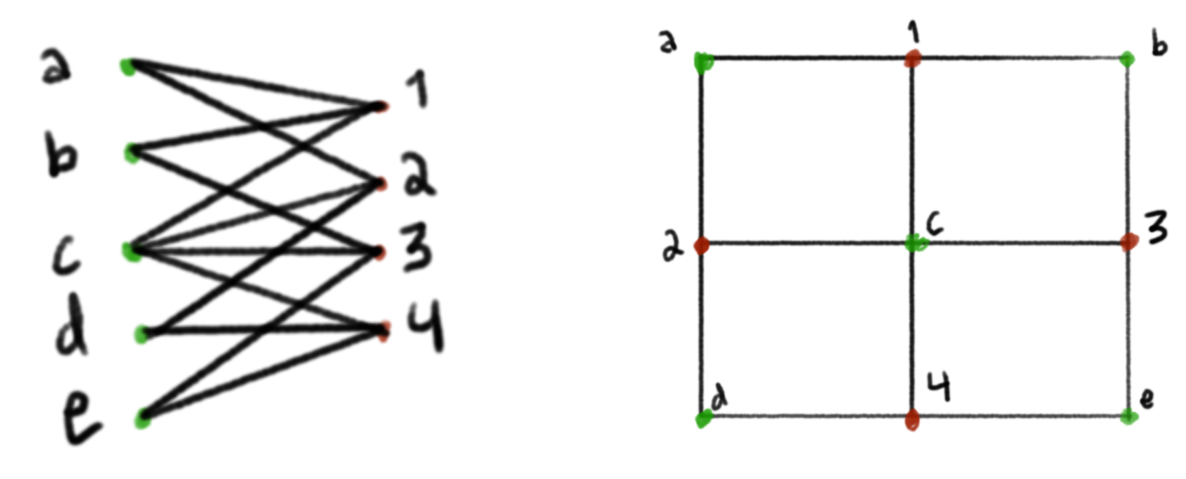
\includegraphics[width=0.66\textwidth]{w12_bigraph}
        \caption{Example \ref{bigraph} of a two ways to express a
            \emph{bigraph}}
    \end{figure}
\end{example}
\begin{definition}[Cubic Graph ($Q_3$)]
    \begin{gather*}
    V=\{0,1\}^3 \quad |V|=8 \\
    E=\{(a_1,b_1,c_1),(a_2,b_2,c_2) \mid |a_1-a_2|+|b_1-b_2|+|c_1-c_2|=1\}
    \end{gather*}
    How we define the two parts of the bigraph:
    \begin{gather*}
        V_1=\{(a,b,c) \mid a+b+c \text{ is even}\} \\
        V_2=\{(a,b,c) \mid a+b+c \text{ is odd}\}
    \end{gather*}
        \begin{figure}[ht]
        \centering
        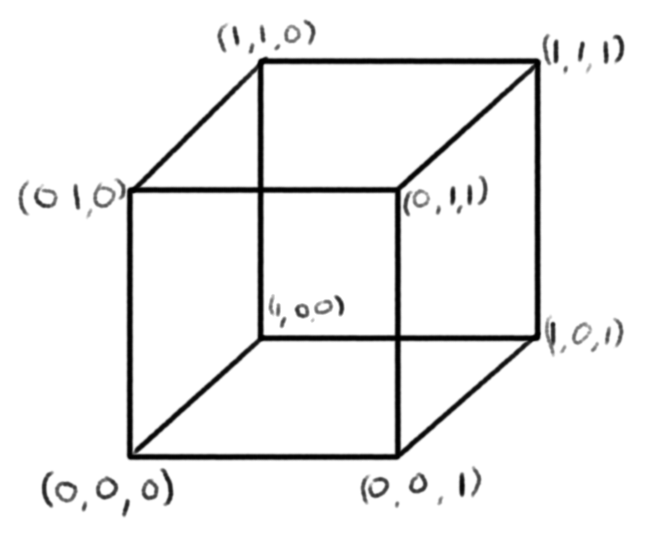
\includegraphics[width=0.33\textwidth]{w12_cubic}
        \caption{Example of a cubic graph}
    \end{figure}
\end{definition}
\begin{definition}[Complete Bigraph ($K_{n,m}$)]
    \begin{gather*}
    |V_1|=m,|V_2|=n \quad V_1 \cap V_2 = \emptyset \\
    E = \{\{v,u\} \mid v \in V_1, u \in V_2\} \\
    |V|=m+n \quad |E|=mn
    \end{gather*}
\end{definition}
\begin{claim}
    In a \emph{bigraph} the number of vertices in a \emph{simple circuit} is
    always even.
\end{claim}
\begin{definition}[Regular Graph]
    A graph $G=(V,E)$ is \emph{$d$-regular} if from all $v \in V$, $\deg(v)=d$.

    For example, $Q_3$ is $3$-regular.
\end{definition}
\begin{claim}
    For a \emph{regular} bigraph, $|V_1|=|V_2|$.
\end{claim}
\begin{proof}
    $$|E|=d\cdot |V_1|=d\cdot |V_2| \implies |V_1|=|V_2|$$
\end{proof}
\section{Special Circuits}
\subsection{Hamiltonian Circuits}

\begin{definition}[Hamiltonian Circuit]
    A \emph{simple circuit} is called a \emph{Hamiltonian circuit} if it passes
    through each vertex of a graph exactly once.

    In other words, $(v_0,v_1,\dots,v_n=v_0)$ is a \emph{Hamiltonian circuit} if
    for all $v \in V$ there exists $1\leq i \leq n$ such that $v_i=v$.
\end{definition}
\begin{claim}
    If $G=(V_1\cup V_2,E)$ is a \emph{bigraph} and $G$ contains a
    \emph{Hamiltonian circuit}, then $|V_1|=|V_2|$.
\end{claim}
\begin{proof}
    We suppose $(v_0,v_1,\dots,v_n=v_0)$ is a \emph{Hamiltonian circuit} where:
    $$v_0 \in V_1 \to v_1 \in V_2 \to v_2 \in V_1 \to v_3 \in V_2 \to\dots$$
    From this we see that $n$ is even and that $|V_1|=|V_2|$.
\end{proof}
\begin{claim}
    For all $n\geq 2$, the graph $Q_n$ contains a \emph{Hamiltonian circuit}.
\end{claim}
\begin{definition}[Hypercube Graph ($Q_n$)]
    \begin{gather*}
    V=\{0,1\}^n \quad |V|=2^n \\
    E=\left\{(a_1,\dots,a_n),(b_1,\dots,b_n) \;\middle|\; \sum_{i=1}^{n}|a_i-b_i|=1\right\}
    \end{gather*}
\end{definition}
\begin{proof}
    We will use proof by induction:
    \begin{enumerate}[I.]
        \item $n=2$
    \begin{figure}[ht]
        \centering
        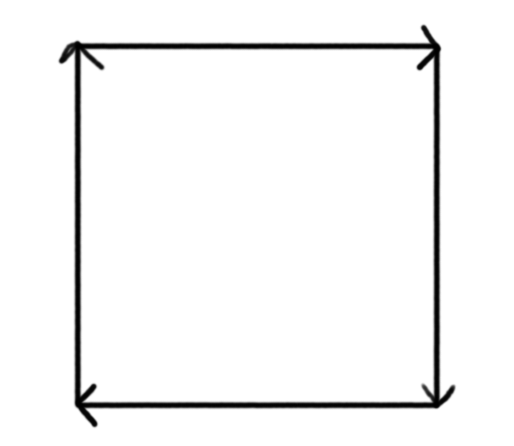
\includegraphics[width=0.2\textwidth]{w12_q2}
        \caption{\emph{Hamiltonian} graph of $Q_2$}
    \end{figure}
        \item We assume correctness on $Q_{n-1}$ and will prove for $Q_n$:
    \begin{gather*}
        A=\{(a_1,a_2,\dots, a_{n-1},0) \mid \forall i \in [n-1], a_i \in\{0,1\}\} \\
        B=\{(a_1,a_2,\dots, a_{n-1},1) \mid \forall i \in [n-1], a_i \in\{0,1\}\} \\
        V=A \cup B
    \end{gather*}
        \begin{figure}[ht]
        \centering
        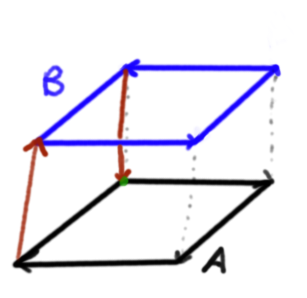
\includegraphics[width=0.33\textwidth]{w12_q3}
        \caption{\emph{Hamiltonian} graph of $Q_3$}
    \end{figure}
    Based on our assumption, $A$ contains the following \emph{Hamiltonian
    circuit}:
    $$(v_0,v_1,\dots,v_{2^{n-1}}=v_0) \quad v_0=(0,0,\dots,0)$$
    And $B$ contains the following \emph{Hamiltonian circuit}:
    $$(u_0,u_1,\dots,u_{2^{n-1}}=u_0) \quad u_0=(0,0,\dots,1)$$
    \begin{note}
        We can go from $v_i$ to $u_i$ by changing the last number from $0$ to $1$.
    \end{note}
    Therefore, we can create the following \emph{Hamiltonian circuit}:
    $$(v_0,v_1,\dots,v_{2^{n-1}-2},v_{2^{n-1}-1},u_{2^{n-1}-1},u_{2^{n-1}-2},\dots,u_2,u_1,u_0,v_0)$$
    Which is a \emph{Hamiltonian circuit} in $Q_n$.
    \end{enumerate}
\end{proof}
\subsection{Eulerian Circuits}
\begin{definition}[Eulerian Circuit]
   Given connected graph $G$, a \emph{circuit} (not necessarily \emph{simple})
   $(v_0,v_1,\dots,v_n=v_0)$ is called an \emph{Eulerian circuit} if for all $e
   \in E$ there exists a single $1\leq i \leq n$ such that $e=\{v_i,v_{i+1}\}$.

   In other words, an \emph{Eulerian circuit} is circuit that visits each edge
   exactly once.
\end{definition}
\begin{example}[Seven Bridges of K\"onigsberg]
    \begin{figure}[ht]
        \centering
        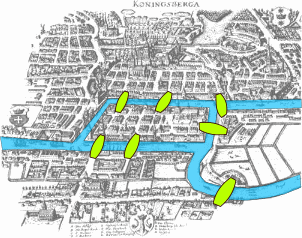
\includegraphics[width=0.33\textwidth]{w12_konigsberg}
        \caption{Map of K\"onigsberg in Euler's time}
    \end{figure}
    The problem was to devise a \emph{circuit} such that one could cross every
    bridge exactly once. Euler proved this to be impossible.
\end{example}
\begin{theorem}
    Given a connected graph $G=(V,E)$, there exists an \emph{Eulerian circuit}
    if and only if for all $v \in V$, $\deg(v)$ is even.
\end{theorem}
\begin{proof}
    Being that we have to prove that this is $\iff$, we must prove both directions:
    \begin{enumerate}
        \item[$\Leftarrow$] Given an \emph{Eulerian circuit}, each visit to a
            vertex adds $2$ to its degree. (This is also true for the vertex
            that we started from because we initially leave from it and must
            return to it in the end)

        \item[$\Rightarrow$] We will prove by induction on the number of edges
            $|E|=m$.
            \begin{enumerate}[I.]
               \item $m=0$ $\checkmark$
               \item We assume the statement holds for less than $m$ edges:

            $G$ is connected, and for all $v \in V$, $\deg(v)$
            is even. Therefore, $G$ does not have any \emph{leaves}, and is
            therefore not a \emph{tree}. And since $G$ is connected but isn't a
            \emph{tree}, we know that it then must contain a \emph{simple
            circuit} $(v_0,v_1,\dots,v_n=v_0)$.

            We define $G'=(V,E')$ as $G$ without all the edges in its
            \emph{simple circuit}. In other words:
            $$E'=E \setminus \{\{v_i,v_{i+1}\} \mid 0 \leq i \leq n-1\}$$
            In $G'$, the degree of each vertex is even. However $G'$ is not
            necessarily connected. We will define $G'$'s \emph{components} as
            $V_1,V_2,\dots,V_l$, where for all $1 \leq i \leq l$: $G_i=(V_i,E_i)$.

            For all $G_i$ the number of edges is less than $m$. Therefore based
            on the assumption of induction, $G_i$ contains a \emph{Eulerian
            circuit}.

            We see that for all $i$: $V_i\cap\{v_0,v_1,\dots,v_{n-1}\}\neq
            \emptyset$. In other words, for each \emph{component} $V_i$, there
            is a representative from the original circuit.

            Given $u \in V_i$, knowing that $G$ is connected, there exists a
            \emph{path} in $G$ between $v_0$ and $u$.
            $$(w_0=v_0,w_1,w_2,\dots,w_n=u)$$
            $$j=\max\{i\mid w_i \in \{v_0,v_1,\dots,v_{n-1}\}\}$$
            We get that all the vertices $w_j,\dots,w_k$ are all in $V_i$, and
            therefore $w_j$ is part of the circuit and it is the representative
            of the circuit in \emph{component} $V_i$.
            We see that we can chose a set of representatives from all of the
            \emph{components} that are all in the set $\{v_0,\dots,v_{n-1}\}$.

            We will now build an \emph{Eulerian circuit} for the graph $G$:
            $$\forall \; 1 \leq i \leq l: f(i)=\min\{i \mid v_i \in V_i\}$$
            We will begin with $v_0$. If there exists an $i$ such that $v_0=f(i)$,
            then we will cover \emph{component} $V_i$ by an \emph{Eulerian
            circuit} that we got from our induction assumption. We now continue
            to $v_1$. If there exists an $i$ such that $v_1=f(i)$ we will cover
            $V_i$ until we come back to $v_1$. Then we can continue to $v_2$
            and so on until $v_n=v_0$.
            \end{enumerate}
    \end{enumerate}
\end{proof}
\section{Ramsey Theory}

Coloring of graph $G=(V,E)$ with $k$ colors $\{c_1,c_2,\dots,c_k\}$ is
essentially a function:
$$C: E \to \{c_1,c_2,\dots,c_k\}$$
We will specifically we working with coloring graphs with two different colors,
namely \textcolor{red}{red} and \textcolor{blue}{blue}.

\begin{claim}
    In coloring $K_6$ (the complete graph with six vertices), with two colors
    \textcolor{red}{red} and \textcolor{blue}{blue}, we will be able to find a
    \textcolor{red}{red $K_3$} or a \textcolor{blue}{blue $K_3$} (or both).
\end{claim}

\begin{proof}
    Suppose $v_0 \in V$. Given that our graph is complete, $\deg(v_0)=5$. By
    the \emph{pigeonhole principle}, there are at least \textcolor{red}{three red
    edges} or \textcolor{blue}{three blue edges} emanating from $v_0$.

    If $v_0$ emits \textcolor{red}{three red edges} we will label the vertices
    they connect to $u_1,u_2,u_3$. If there is $1 \leq i < j \leq 3$ such that
    $(u_i,u_j)$ is \textcolor{red}{red} then $v_0,u_i,u_j$ forms a
    \textcolor{red}{red $K_3$}. If there aren't any, then we know that
    $u_1,u_2,u_3$ forms a \textcolor{blue}{blue $K_3$}.

    Likewise, if $v_0$ emits \textcolor{blue}{three blue edges}, the same can
    be said in reverse.
\end{proof}

\begin{definition}[Ramsey's theorem]
    Given $s,t \in \mathbb{N}$, $R(s,t)$ is the smallest $n$ such that when
    coloring $K_n$ in \textcolor{red}{red} or \textcolor{blue}{blue}, at least
    one of the following cases is true:
    \begin{enumerate}[a.] \tightlist
        \item There is $S \subset V$, $|S|=s$ such that all edges between the
            vertices in $S$ are \textcolor{red}{red}.
        \item There is $T \subset V$, $|T|=t$ such that all edges between the
            vertices in $T$ are \textcolor{blue}{blue}.
    \end{enumerate}
    In other words there is guaranteed to be a \textcolor{red}{red $K_s$} or a
    \textcolor{blue}{blue $K_t$} (or both).
\end{definition}
From our previous claim, $R(\textcolor{red}{3},\textcolor{blue}{3}) \leq 6$.
How can we prove that $R(\textcolor{red}{3},\textcolor{blue}{3})= 6$?
    \begin{figure}[ht]
        \centering
        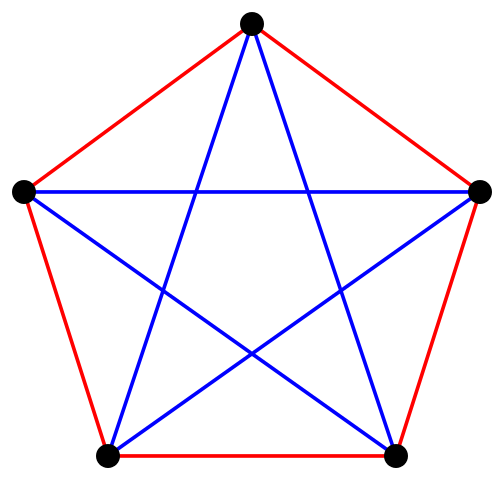
\includegraphics[width=0.33\textwidth]{w12_k5}
        \caption{A coloring of $K_5$ with no monochromatic $K_3$}
    \end{figure}

Since $R(\textcolor{red}{3},\textcolor{blue}{3}) \neq 5$,
$R(\textcolor{red}{3},\textcolor{blue}{3}) = 6$.

For all $s,t$:
\begin{itemize} \tightlist
    \item $R(1,t) = 1$
    \item $R(s,1) = 1$
    \item $R(2,t) = t$
    \item $R(s,2) = s$
    \item $R(4,4) = 18$
    \item $R(5,5) = \text{still unknown!}$
\end{itemize}
\begin{lemma}
    For all $m,n \in \mathbb{N}$:
    $$R(n,m)\leq \underbrace{R(n-1,m)}_{a}+\underbrace{R(n,m-1)}_{b}$$
\end{lemma}
\begin{proof}
    For all colorings of $K_{a+b}$ in \textcolor{red}{red} or
    \textcolor{blue}{blue} we are guaranteed that there will be either a
    \textcolor{red}{red $K_n$} or a \textcolor{blue}{blue $K_m$}.

    Suppose $v \in V$. $v$ emits $a+b-1$ edges. We are guaranteed one of the
    following cases:
    \begin{enumerate}[a.] \tightlist
        \item From $v$ emanates \textcolor{red}{$a$ red edges}.
        \item From $v$ emanates \textcolor{blue}{$b$ blue edges}.
    \end{enumerate}
    Suppose that case "a" is true:

    We look at the $a$ neighbors that are connected to $v$ by
    \textcolor{red}{red edges}. We are guaranteed that between then there
    exists either a \textcolor{red}{red $K_{n-1}$} or a \textcolor{blue}{blue
    $K_m$}. If there's a \textcolor{blue}{blue $K_m$}, we're done. Otherwise
    there's a \textcolor{red}{red $K_{n-1}$} and we'll join $v$ to them to
    create a \textcolor{red}{red $K_{n}$}.

    If case "b" is true:

    We look at the $a$ neighbors that are connected to $v$ by
    \textcolor{blue}{blue edges}. We are guaranteed that between then there
    exists either a \textcolor{red}{red $K_{n}$} or a \textcolor{blue}{blue
    $K_{m-1}$}. If there's a \textcolor{red}{red $K_n$}, we're done. Otherwise
    there's a \textcolor{blue}{blue $K_{m-1}$} and we'll join $v$ to them to
    create a \textcolor{blue}{blue $K_{m}$}.
\end{proof}
\begin{example}
    $$R(3,4) \leq 10$$
    From our lemma:
    $$R(3,4) \leq R(2,4)+R(3,3) = 4+6=10$$
\end{example}
\begin{theorem}
    $$R(n,m) \leq \binom{n+m-2}{m-1}$$
\end{theorem}
\end{document}
